\chapter{Volatility}
\label{chapter:volatility}
As mentioned, volatility is a measure of the uncertainty of future stock price movements. In other words, a higher volatility will lead to greater future fluctuations in the stock price, whereas a stock with lower volatility is more stable. This phenomenon is exemplified in \autoref{fig:VarVol}, where we can see the greater fluctuations of the high-volatility process (red) compared to the much smaller variations of the low-volatility process (orange).
\begin{figure}[!htb]
    \centering
      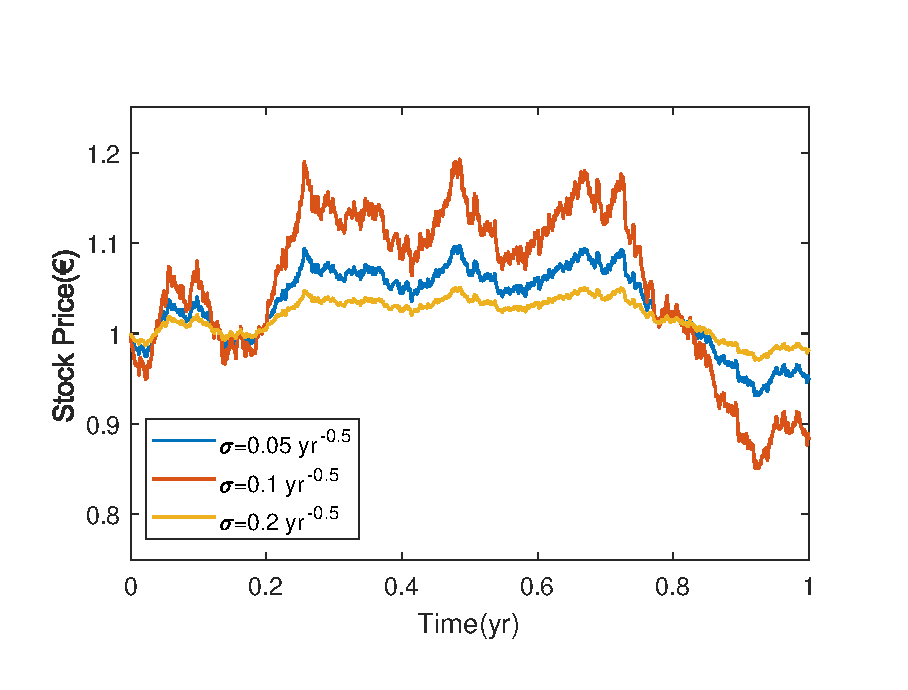
\includegraphics[width=.65\columnwidth]{VarVol.eps}
      \caption[Example of three identical GBM processes with different volatilities]{Example of three identical GBM processes with maturity $T=\SI{1}{\year}$, interest rate $r=\SI{0.01}{\per\year}$ and initial stock price $S_0=\SI{1}{\EUR}$. The volatilities are $\sigma=\SI{0.05}{\year\tothe{-1/2}}$, $\sigma=\SI{0.1}{\year\tothe{-1/2}}$ and $\sigma=\SI{0.2}{\year\tothe{-1/2}}$ for the orange, blue and red plot lines represented, respectively. To emphasize this effect, the underlying Brownian Motion $W(t)$ used to generate all three paths was the same.}\label{fig:VarVol}
    \end{figure}

Of all the parameters in the BS formula (eq.\eqref{BS2}), volatility is the only one we can't easily measure from market data.
Furthermore, unlike the interest rate, volatility has a great impact on the behavior of stock prices and, consequently, on the price of options~\cite{Wilmott3}.
These two factors make volatility one of the most important subjects in all of mathematical finance and thus the focus of much research.

Usually, volatility is estimated from the standard deviation of the rate of returns~\cite{Hull}.
We begin by measuring the stock price at fixed time intervals (e.g. daily, monthly), such that $S_i$ corresponds to the stock price at the end of the $i$th interval. We define the return rate, $u_i$, as
\begin{equation}
u_i=\log\left(\frac{S_i}{S_{i-1}}\right).
\end{equation}
We can then calculate the standard deviation of this rate, $s$, with the classical formula
\begin{equation}
s=\sqrt{\frac{1}{n-1}\sum_{i=1}^n(u_i-\overline{u})^2},
\end{equation}
\noindent assuming we have $n+1$ observations and denoting $\overline{u}$ as the average value of the return rates.
The volatility (measured yearly) is given by
\begin{equation}
\sigma=\frac{s}{\sqrt{\tau}}
\end{equation}
\noindent where $\tau$ defines the time interval length measured in years.
The volatility can also be measured in other time periods: we can define a monthly or a daily volatility, but these are less common and will therefore not be used.

Our goal is to model the volatility of any given stock price.
We begin by introducing the implied volatility, crucial to fully grasp the concepts used later. Afterwards, we will introduce four models to replicate market volatility: one with local volatility (Dupire's formula) and three with stochastic volatility (Heston, Static/Dynamic SABR).
Other very common models exist. The GARCH model (Generalized Autoregressive Conditional Heteroskedasticity) along with all its many variations (EGARCH, NGARCH, ...) is particularly popular among econometricians. However, this model is mostly used to forecast volatility, and performs poorly when used to price derivatives~\cite{chourdakis}. Because pricing is our objective, GARCH will not be covered in this work. We will also study the constant volatility model, as used by Black \textit{et al.}, as a benchmark for the quality of our models.



\section{Implied Volatility}
\label{section:impliedvolatility}
\emph{Implied volatility} can be described as the value of stock price volatility that, when input into the BS pricer in eq.\eqref{callputBS}, outputs a value equal to the market price of a given option.
In other words, it would be the stock price volatility that the seller/buyer of the option used when pricing it (assuming the BS model was used).

Because eq.\eqref{callputBS} is not invertible, we need to use some numerical procedure (e.g. Newton's method) to find the value of implied volatility that matches the market and model prices, i.e. we must find, numerically, the solution to the equation
\begin{equation}\label{impvolform}
C(\sigma_{imp})-C_{\mathrm{mkt}}=0,
\end{equation}
\noindent where $C(\sigma_{imp})$ corresponds to the result of eq.\eqref{callputBS} using $\sigma_{imp}$ as (implied) volatility and $C_{\mathrm{mkt}}$ to the price of the option observed in the market.

Because eq.\eqref{callputBS} is monotonic w.r.t. the volatility, we can obtain the implied volatility of an option from its price and vice versa. This duality is so fundamental that investors often disclose options by providing their implied volatility instead of their price~\cite{Wilmott}, as is indeed the case for the data we will use later.

One important property of implied volatility is that, in the real-world, it depends on the strike price and the maturity. This should not occur in the "Black-Scholes world". Because the volatility is a property of the stock, if investors really used the the BS model to price their options, two options with the same underlying stock should have the same implied volatility, regardless of their strike prices or maturities (i.e. the same stock can't have two different volatilities at the same time).
However, when observing real market data, this is in fact what is observed.
The implied volatilities' dependence on the strike price can take one of two forms, known as \emph{smile} and \emph{skew}.
An implied volatility smile presents higher volatilities for options with strikes farther from the current stock price (i.e. the shape of a smile). A skew, on the other hand, only presents higher volatilities in one of these directions (i.e. only for strikes either greater or smaller than the current stock price). Both phenomena are represented in \autoref{fig:smileskew}.
\begin{figure}[!htb]
  \begin{subfigmatrix}{2}
    \subfigure[Smile]{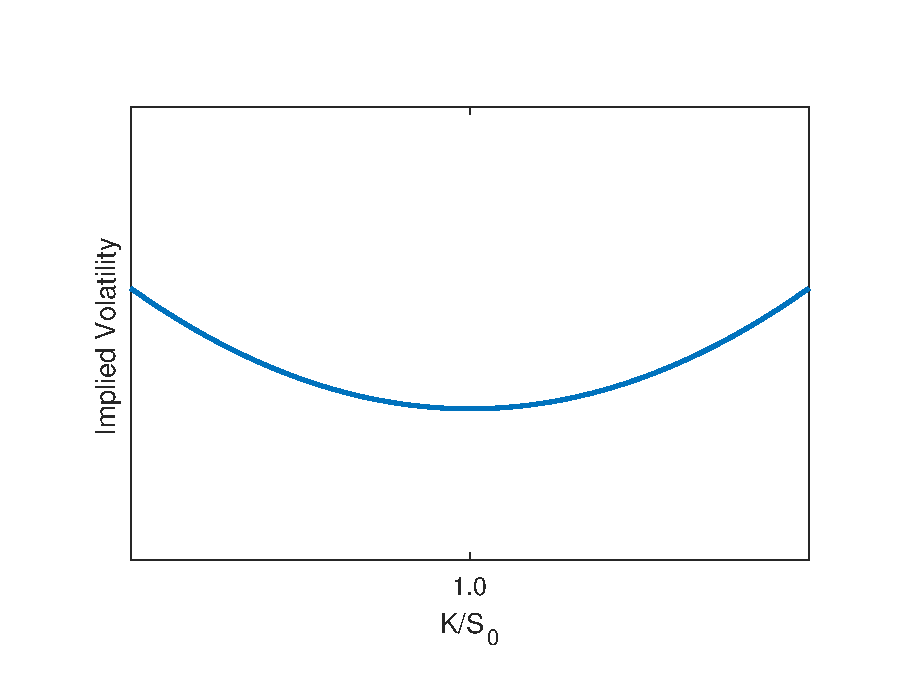
\includegraphics[width=0.49\linewidth]{Smile.eps}}
    \subfigure[Skew]{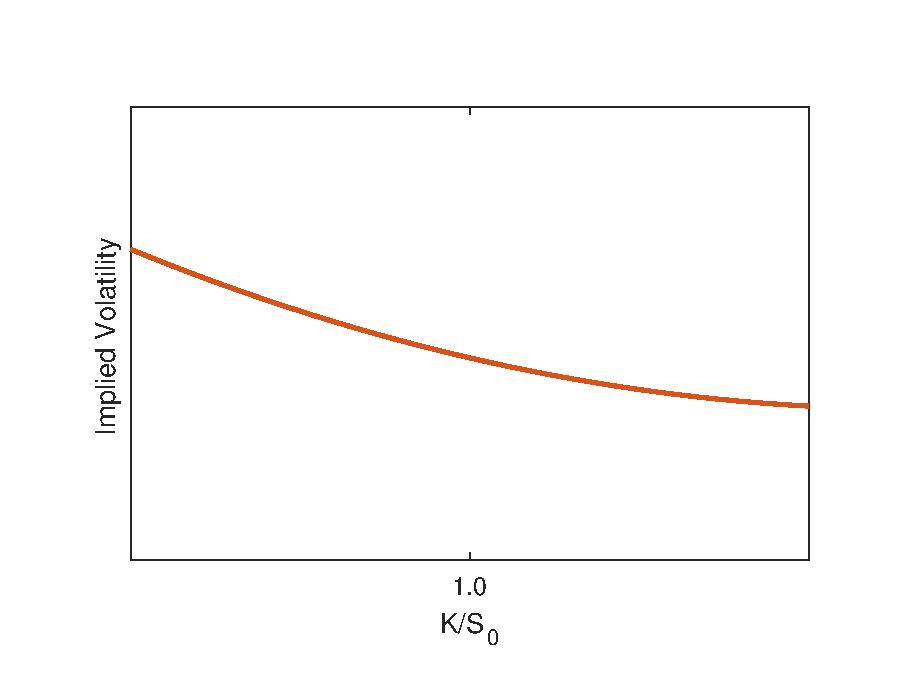
\includegraphics[width=0.49\linewidth]{Skew.eps}}
  \end{subfigmatrix}
  \caption[Representation of the implied volatility smile and skew functions.]{Representation of the implied volatility smile (left) and skew (right) functions.}
  \label{fig:smileskew}
\end{figure}


Because of their higher implied volatility, we can conclude that, if we observe a smile in the data, options with strikes different from the current stock price are \emph{overpriced}.
The reason behind this odd market behavior is related to the simple demand-supply rule~\cite{Wilmott3}. On the one hand, some investors are risk-averse and want to hedge their losses in case of a market crash (as explained in subsection \ref{subsection:why options are important}). They don't mind paying a higher price for an option if this means they would be relatively safe from potentially devastating market crashes. For this reason, the prices of call options with lower strikes increase, driving their implied volatility up. On the other hand, other investors are risk-seekers and want to take advantage of possible sudden price movements, buying the stocks for the lower strike prices. They don't mind paying higher prices for the chance of earning high profits and this drives the prices of high strike call options (and, consequently, their implied volatility) up. This fear-greed duality gives rise to the observed volatility smile. 
In the case of the volatility skew, only one of the two fenomena described occurs.


The presence of a smile in the data instead of a skew, and vice-versa, is determined by the type of product serving as underlying asset - Forex market options usually exhibit volatility smiles whereas index and commodities options usually show a volatility skew.

The dependence of the implied volatility on the maturity date is more complex, but in general it decreases with $T$.

It can also be shown that the implied volatility is the same for calls and puts~\cite{Hull}, though the causes of the volatility smile/skew for put options are the opposite of the ones described before, for calls.



We saw in eq.\eqref{impvolform} that the implied volatility depends on the option's market price. As we will see in later sections, it is quite important to visualize this relation. Therefore we present in \autoref{fig:ImpVolPrice} the implied volatility functions w.r.t. the option's market price for three different strike prices.


\begin{figure}[!htb]
    \centering
      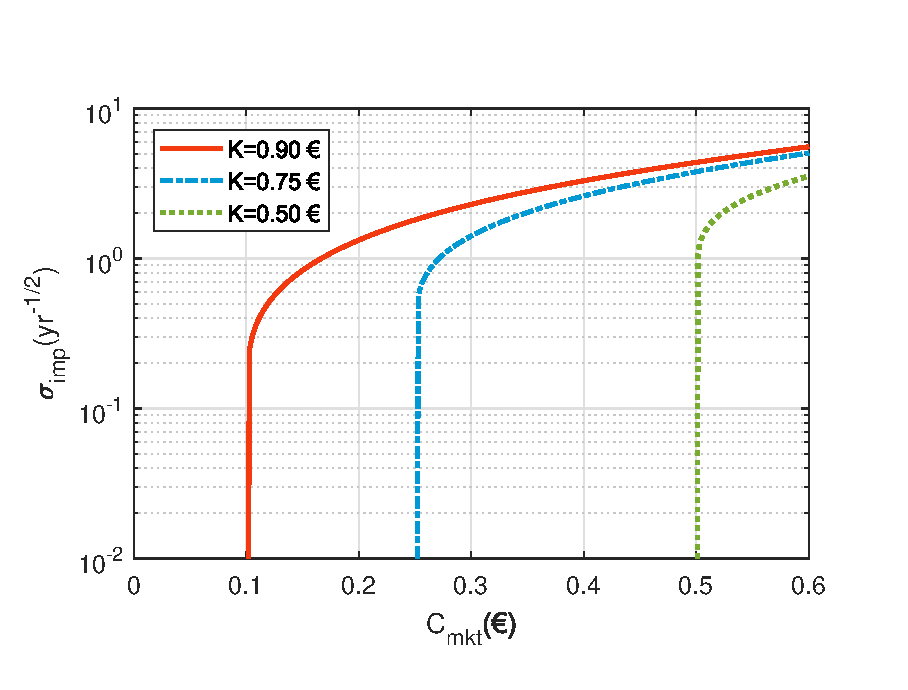
\includegraphics[width=.65\columnwidth]{ImpVolC.eps}
      \caption[Relationship between the implied volatility and the price of a call option.]{Relationship between the implied volatility and the price of a call option. The parameters used were $T=21$ days, interest rate $r=\SI{0.01}{\per\year}$ and initial stock price $S_0=\SI{1}{\EUR}$. The stike prices are $K=\SI{0.9}{\EUR}$, $K=\SI{0.75}{\EUR}$ and $K=\SI{0.5}{\EUR}$ for the red full line, the blue dot-dashed line and the green dot-dashed line, respectively.}\label{fig:ImpVolPrice}
    \end{figure}

We can see that the implied volatility goes to zero extremely fast when we approach the lower bound of the call option's price, $S_0-Ke^{-rT}$ (from eq.\eqref{bound}) - the lower bounds for the option prices with strikes $K=\SI{0.9}{\EUR}$, $K=\SI{0.75}{\EUR}$ and $K=\SI{0.5}{\EUR}$ are, respectively, $C=\SI{0.1007}{\EUR}$, $C=\SI{0.2506}{\EUR}$ and $C=\SI{0.5004}{\EUR}$). We can also observe that this property is more pronounced for lower strikes. This observation will become very important in later sections.




\section{Local Volatility}
\label{section:localvolatility}
In their original work, Black \textit{et al.} assumed that volatility is constant throughout the whole option duration. From market data, it can be clearly seen that this is not the case~\cite{DJIA}. There may be times where new information reaches the market  (e.g. the results of an election) and trading increases, driving volatility up. It is equally true that shortly before this information is known, trading may stall due to expectancy, and volatilities go down. 

The constant volatility BS model is therefore clearly incapable of completely grasping real-world trading. We should use a model where volatility is dynamic, measuring the uncertainty on the stock price movement at any point in time.
However, as we saw in section \ref{section:impliedvolatility}, the market's view of volatility also depends on the strike price.
The volatility should therefore be a function of both time and stock price: $\sigma(S,t)$. We call this model \emph{local volatility} and the geometric Brownian motion from eq. \ref{GBM} is transformed into
\begin{equation}\label{GBM2}
dS(t)=rS(t)dt+\sigma(S,t)S(t)dW(t),
\end{equation}
\noindent where $\sigma(S,t)$ is some function of $S$ and $t$.


This local volatility model implies that we have a nonlinear \emph{deterministic} volatility surface, $\sigma(S,t)$, which can be thought of as the market's expectation of future volatility at time $t$ if the stock price is $S$ at that time.



Because we can't directly measure the local volatility of a stock from market data, we need some models to find it. One of the most used of these is known as Dupire's formula.


\subsection{Dupire's model}
\label{subsection:Dupire}
One of the most famous results in the modelling of the local volatility function was obtained by Dupire~\cite{Dupire}. In his article, this author derives a theoretical formula for $\sigma(S,t)$, given by
\begin{equation}\label{dupire}
\sigma(S,t)=\sqrt{\frac{\displaystyle\pdv{C}{T}+rS\pdv{C}{K}}{\displaystyle\frac{1}{2}S^2\pdv{^2C}{K^2}}},
\end{equation}
\noindent where $C=C(K,T)$ is the price of an European call option with strike price $K$ and maturity $T$. All the derivatives are evaluated at $K=S$ and $T=t$.



\begin{proof}

We begin by assuming that the stock price $S$ follows a dynamic transition probability density function $p(S(t),t,S'(t'),t')$. In other words, by integrating this density function we would obtain the probability of the stock price reaching a price $S'$ at a time $t'$ having started at $S$ at time $t$.

The present value of a call option, $C(S,t,K,T)$, can be deduced as its expected future payoff, discounted backwards in time, which results in
\begin{equation}
\begin{split}\label{deriv0}
C(K,T)=e^{-r(T-t)}\mathbb{E}\left[\max\left(S'-K,0\right)\right]&=e^{-r(T-t)}\int_0^\infty\max\left(S'-K,0\right)p(S,t,S',T)dS'\\
&=e^{-r(T-t)}\int_K^\infty(S'-K)p(S,t,S',T)dS'.
\end{split}
\end{equation}
Taking the first derivative of this result with respect to the strike price $K$, we obtain
\begin{equation}\label{dcdk}
\pdv{C}{K}=-e^{-r(T-t)}\int_K^\infty p(S,t,S',T)dS'.
\end{equation}
The second derivative results in
\begin{equation}\label{d2cdk2}
\pdv{^2C}{K^2}=e^{-r(T-t)}p(S,t,K,T).
\end{equation}
\noindent assuming $p(S,t,\infty,T)=0$.

We now make a brief detour to derive the Fokker-Planck equation (following the procedure shown in \cite{Wilmott}), which we require for the next steps.
We begin by assuming a trinomial model: at each time step, our stock price can only increase or decrease by an amount $dS$, with probabilities $\phi^+$ and $\phi^-$, respectively, or remain the same, with probability $(1-\phi^+-\phi^-)$.
The expected value of the change is therefore
\begin{equation}
\phi^+dS+(1-\phi^+-\phi^-).0+\phi^-(-dS)=dS(\phi^+-\phi^-),
\end{equation}
\noindent and its variance is approximately given by
\begin{equation}
(dS)^2(\phi^++\phi^--(\phi^+-\phi^-)^2)\approx (dS)^2(\phi^++\phi^-)
\end{equation}
\noindent where we take only the first order terms. The expected value of the change of a GBM can be thought of as its drift term (i.e. $rSdt$), and the variance is its stochastic term squared (i.e. $(\sigma SdW)^2=\sigma^2S^2dt$), so that we have
\begin{equation}
\begin{split}
rSdt&=(\phi^+-\phi^-)dS;\\
\sigma^2S^2dt&=(\phi^++\phi^-)(dS)^2,
\end{split}
\end{equation}
\noindent from which we can derive the probabilities $\phi^+$ and $\phi^-$ as
\begin{equation}
\begin{split}
\phi^+&=\frac{1}{2}\frac{dt}{dS^2}(rSdS+\sigma^2S^2);\\
\phi^-&=\frac{1}{2}\frac{dt}{dS^2}(-rSdS+\sigma^2S^2).
\end{split}
\end{equation}

We can now move backwards and derive the probability of reaching the price $S'$ at time $t'$ having started at the previous time $t'-dt$ with some (unknown) price $S$, which could be either $S'+dS$, $S'-dS$ or $S'$ (assuming a trinomial movement). This probability is indeed the probability density, $ p(S,t,S',T) $ and can be derived as
\begin{equation}
p(S,t,S',T)=\phi^-p(S'+dS,t-dt,S',T)+(1-\phi^+-\phi^-)(S',t-dt,S',T)+\phi^+p(S'-dS,t-dt,S',T).
\end{equation}
\noindent If we expand each term on its Taylor series around point $(S',t')$, we get
\begin{equation}
\begin{split}
p(S,t,S',T)=&\ \phi^-\left(p(S',t,S',T)+dS\frac{dp}{dS'}+\frac{1}{2}(dS)^2\frac{d^2p}{dS^2}-dt\frac{dp}{dt'}\right)\\
&+(1-\phi^+-\phi^-)\left(p(S',t,S',T)-dt\frac{dp}{dt'}\right)\\
&+\phi^+\left(p(S',t,S',T)-dS\frac{dp}{dS'}+\frac{1}{2}(dS)^2\frac{d^2p}{dS^2}-dt\frac{dp}{dt'}\right)\\
=&\frac{1}{2}\frac{dt}{dS'^2}\sigma^2S'^2(dS)^2\frac{d^2p}{dS'^2}-\frac{dt}{dS'^2}rS'(dS)^2\frac{dp}{dS'},
\end{split}
\end{equation}
\noindent from which we can derive the famous Fokker-Planck equation (with rather sloppy notation) as
\begin{equation}\label{FokkerPlanck}
\pdv{p}{T}=\frac{1}{2}\pdv{^2(\sigma^2S'^2p)}{S'^2}-\pdv{(rS'p)}{S'}.
\end{equation}
\noindent where we have used $t'=T$.


From eq. \ref{deriv0} we can easily derive
\begin{equation}
\pdv{C}{T}=-rC+e^{-r(T-t)}\int_K^\infty(S'-K)\pdv{p}{T}dS'.
\end{equation}
Using eq. \ref{FokkerPlanck}, we can transform this relation into
\begin{equation}
\pdv{C}{T}=-rC+e^{-r(T-t)}\int_K^\infty(S'-K)\left(\frac{1}{2}\pdv{^2(\sigma^2S'^2p)}{S'^2}-r\pdv{(S'p)}{S'}\right)dS'.
\end{equation}

We now split the terms in the integral to evaluate them independently. We integrate the second term by parts as
\begin{equation}
\begin{split}
\int_K^\infty(S'-K)\left(-r\pdv{(S'p)}{S'}\right)dS'&=-r(S'-K)(S'p)\big|_{S'=K}^\infty+r\int_K^\infty S'p dS'\\
&=r\int_K^\infty (S'-K)p dS'+rK\int_K^\infty p dS'\\
&=e^{r(T-t)}rV-rK\pdv{C}{K}
\end{split}
\end{equation}
\noindent where in the first step we assumed that $p$ and its first derivative w.r.t. $S$ go sufficiently fast to zero and in last step we used eqs.\eqref{deriv0} and \eqref{dcdk}.

Turning now to the first term of the integral, we integrate twice by parts
\begin{equation}
\begin{split}
\int_K^\infty(S'-K)\left(\frac{1}{2}\pdv{^2(\sigma^2S'^2p)}{S'^2}\right)dS'&=\frac{1}{2}(S'-K)\pdv{(\sigma^2S'^2p)}{S'}\bigg|_{S'=K}^\infty-\frac{1}{2}\int_K^\infty\left(\pdv{(\sigma^2S'^2p)}{S'}\right)dS'\\
&=\frac{1}{2}\sigma^2S'^2p\big|_{S'=K}^\infty=\frac{1}{2}\sigma^2(K,T)K^2p(S,t,K,T)\\
&=\frac{1}{2}e^{r(T-t)}\sigma^2(K,T)K^2\pdv{^2C}{K^2},
\end{split}
\end{equation}
\noindent where in the last step we used eq.\eqref{d2cdk2} and again assumed that $p$ goes to zero sufficiently fast.

Collecting all the terms, we obtain
\begin{equation}
\pdv{C}{T}=\frac{1}{2}\sigma^2(K,T)K^2\pdv{^2C}{K^2}-rK\pdv{C}{K}.
\end{equation}
\noindent from which, by rearranging all the terms and applying the variable change $\sigma(K,T)\implies \sigma(S,t)$, we get
\begin{equation}
\sigma(S,t)=\sqrt{\frac{\displaystyle\pdv{C}{T}+rS\pdv{C}{K}}{\displaystyle\frac{1}{2}S^2\pdv{^2C}{K^2}}}.
\end{equation}
\noindent assuming all the derivatives are evaluated at $K=S$ and $T=t$.

\end{proof}

As can be seen, we need to differentiate the option prices with respect to their strikes and maturities. To achieve this, we need first to gather, from the market, a large number of prices for options with different maturities and strikes. We then implement some interpolation on these values to obtain an option price surface (with $K$ and $T$ as variables). Finally, we calculate the gradients of this interpolated surface and input them into eq.\eqref{dupire} to obtain the local volatility surface.
We can then sample the local volatility at each time step of our simulation.


A major problem can be pointed out in eq.\eqref{dupire}. For options far in or far out of the money (i.e. with strikes much greater or much smaller that $S_0$), it can be shown that the option price depends almost linearly on the strike. This means that the second derivative of the price w.r.t. the strike is very small in these regions. Because this value is in the denominator of eq.\eqref{dupire}, the local volatility will explode in such cases, which is unrealistic.


One possible solution to this problem is to relate our local volatility with the implied volatility surface instead of the option price's~\cite{Wilmott2}.
The relation obtained is
\begin{equation}\label{dupire2}
\boxed{\sigma(S,t)=\sqrt{\frac{\displaystyle\sigma_{imp}^2+2t\sigma_{imp}\pdv{\sigma_{imp}}{T}+2rSt\sigma_{imp}\pdv{\sigma_{imp}}{K}}{\displaystyle\left(1+Sd_1\sqrt{t}\pdv{\sigma_{imp}}{K}\right)^2+S^2t\sigma_{imp}\left(\pdv{^2\sigma_{imp}}{K^2}-d_1\left(\pdv{\sigma_{imp}}{K}\right)^2\sqrt{t}\right)}},}
\end{equation}
\noindent where $d_1$ is given by
\begin{equation}
d_1=\frac{\log(S_0/S)+\left(r+\frac{1}{2}\sigma_{imp}^2\right)t}{\sigma_{imp}\sqrt{t}},
\end{equation}
\noindent with $S_0$ being the stock price at $t=0$. We define $\sigma_{imp}=\sigma_{imp}(K,T)$ as the implied volatilities of options with maturity $T$, and strike $K$. Furthermore, $\sigma_{imp}$ and all its derivatives are evaluated at $K=S$ and $T=t$. This formula can be obtained from eq.\eqref{dupire} by applying the transformation from call prices to implied volatilities.


We now need to generate the implied volatility surface from market data in order to find the gradients shown in eq.\eqref{dupire2}. We again need to interpolate between the market's implied volatilities in order to find this surface.
However, because we only have access to market data for a finite set implied volatilities, finding the implied volatility surface requires some form of interpolation and extrapolation. This problem is therefore very much ill-posed (i.e. a small change in the input generates a very different output) and the local volatility surface might look unrealistic~\cite{Wilmott}. Furthermore, it depends heavily on the interpolation/extrapolation method chosen, which is problematic.

Because we are directly using the market data, the implied volatility surface is nonparametric and therefore no fitting procedure is required. To ease the problem of ill-posedness, we could heuristically choose some functions to model this surface, fitting their parameters to better replicate the market data, and finally replacing these functions in eq.\eqref{dupire2}, as done by Dewynne~\cite{dewynne}. However, this solution depends heavily on the functions chosen and will not be considered.



Three other problems can be identified in Dupire's local volatility assumption, however.
First, it can be shown that the local volatility surface changes with time~\cite{Wilmott}. This means that the whole interpolation procedure must be done regularly in order for the model to work properly.
Secondly, some authors have pointed out that the volatility smile obtained from Dupire's local-volatility model doesn't follow real market dynamics~\cite{Hagan}: it can be shown that when the price of the stock either increases or decreases, the volatility smile predicted by Dupire's model shifts in the opposite direction. The minimum of the volatility smile would therefore be offset and no longer correspond to the local stock price. The volatility smile dynamics obtained from the local-volatility model would thus be actually worse than if we assumed a constant volatility.
Finally, the gradients used in eq.\eqref{dupire2} have to be generated numerically. This numerical differentiation is very unstable, especially when done on our rough interpolated surface, which might lead to errors in the local volatility obtained.

Despite its problems, Dupire's formula is still very much used by practitioners and performs surprisingly well, as we will see in later chapters.



\section{Stochastic Volatility}
\label{section:stochastic volatility}
As stated before, the volatility is not constant, is not observable and is not predictable, despite our attempts to model it. This seems to indicate that volatility is itself also a stochastic process. Some research has been done into this hypothesis, and many models have been developed to replicate real-world volatilities.

As before, we assume that the stock price follows a geometric Brownian motion
\begin{equation}\label{stochvol}
dS(t)=rS(t)dt+\sigma(S,t)S(t)dW_1(t),
\end{equation}
\noindent but we further hypothesize that the volatility follows
\begin{equation}
d\sigma(S,t)=p(S,\sigma,t)dt+q(S,\sigma,t)dW_2(t),
\end{equation}
\noindent where $p(S,\sigma,t)$ and $q(S,\sigma,t)$ are some functions of the stock price $S$, time $t$ and of the volatility $\sigma$ itself. We also assume that $W_1$ and $W_2$ are two Brownian motion processes with a correlation of $\rho$, i.e.
\begin{equation}
dW_1dW_2=\rho dt.
\end{equation}
\noindent This correlation factor $\rho$ can be explained by the relationship between prices and volatilities~\cite{chourdakis}. Historically, we can see that high volatility periods usually occur when the market is under stress due to low returns (i.e. stock prices decrease). Examples of such periods occurred during the Gulf War in 1991 and during the invasion of Iraq in 2003.
On the other hand, whenever the market stabilizes and returns increase, the volatility goes down.
These factors seem to indicate the existence of a negative correlation between stock prices and volatilities. Thus, to fully grasp market behavior, this correlation must be taken into account.



Choosing the appropriate functions $p(S,\sigma,t)$ and $q(S,\sigma,t)$ is very important since the whole evolution of the stock price depends on them. All stochastic volatility models present a different version of these functions, and each may be more adequate for some types of assets. Furthermore, these functions have some parameters that we have to calibrate in order to best fit our model to market data, as we will see later.


Many stochastic volatility models exist, such as Hull-White~\cite{hullwhite} and Stein-Stein~\cite{stein}. However, the \emph{Heston} model is by far the most popular of these~\cite{chourdakis}.
Another model, known as \emph{SABR}, is also widely used by practitioners, especially in the interest rate derivative markets (i.e. derivatives whose underlying asset is an interest rate). For these reasons, both these models will be studied in detail in this work.


\subsection{Heston Model}
One of the most popular stochastic volatility models is known as \emph{Heston model}. It was developed in 1993 by Steven Heston~\cite{Heston} and it states that stock prices satisfy the relations
\begin{equation}\label{hestons}
\boxed{dS=rSdt+\sqrt{\nu}SdW_1,}
\end{equation}
\begin{equation}\label{hestonv}
\boxed{d\nu=\kappa(\overline{\nu}-\nu)dt+\eta\sqrt{\nu}dW_2,}
\end{equation}
\noindent with $\nu$ corresponding to the stock price variance (i.e. $\nu=\sigma^2$) and again where $W_1$ and $W_2$ have a correlation of $\rho$. We furthermore define $\nu_0$ as the initial variance (i.e. variance at time $t=0$). The original model used a drift parameter $\mu$ instead of the risk-free measure drift $r$ presented here, but a measure transformation, using Gisarnov's theorem, can be easily implemented~\cite{rouah}.

The parameters $\kappa$, $\overline{\nu}$ and $\eta$ are, respectively, the \emph{mean-reversion rate} (i.e. how fast the volatility converges to its mean value), the \emph{long-term variance} (i.e. the mean value of variance) and the \emph{volatility of volatility} (i.e. how erratic is the volatility process).



One of the reasons why the Heston model is so popular is the fact that there exists a closed-form solution for the prices of European options priced under this model. This closed form solution is given by
\begin{equation}\label{CH}
\begin{split}
C_{H}(\theta;K,T)&=e^{-rT}\mathbb{E}\left[\left(S(T)-K\right)\mathbbm{1}_{\left\{S(T)>K\right\}}\right]\\
&=e^{-rT}\left(\mathbb{E}\left[S(T)\mathbbm{1}_{\left\{S(T)>K\right\}}\right]-K\mathbb{E}\left[\mathbbm{1}_{\left\{S(T)>K\right\}}\right]\right)\\
&=S_0P_1-e^{-rT}KP_0,
\end{split}
\end{equation}
\noindent where $C_{H}(\theta;K,T)$ corresponds to the theoretical European call option price under the Heston model, assuming a parameter set $\theta$, strike $K$ and maturity $T$. The variables $P_1$ and $P_2$ are given by
\begin{equation}\label{P1}
P_1=\frac{1}{2}+\frac{1}{\pi}\int_0^\infty\operatorname{Re}\left(\frac{e^{-iu\log K}}{iuS_0e^{rT}}\phi(\theta;u-i,T)\right)du,
\end{equation}
\begin{equation}\label{P2}
P_0=\frac{1}{2}+\frac{1}{\pi}\int_0^\infty\operatorname{Re}\left(\frac{e^{-iu\log K}}{iu}\phi(\theta;u,T)\right)du,
\end{equation}
\noindent where $i$ is the imaginary unit and $\phi(\theta;u,t)$ is the characteristic function of the logarithm of the stock price process - the characteristic function of a random variable is the Fourier transform of the probability density function of that variable.


It is crucial to find the appropriate characteristic function $\phi(\theta;u,t)$ in order to evaluate the integrals in eqs.\eqref{P1} and \eqref{P2} and with them find the option price with eq.\eqref{CH}. In his original article, Heston proposed a solution to this very characteristic function~\cite{Heston}. However, some posterior authors demonstrated that, for large maturities, some discontinuities appeared for the proposed equation~\cite{Kahl}. One possible alternative, proposed by Schoutens~\cite{Schoutens}, avoids this shortcoming and is given by
\begin{equation}\label{charfuncschoutens}
\phi(\theta;u,t)=\exp\left\{iu\left(\log S_0+rt\right)+\frac{\kappa\overline{\nu}}{\eta^2}\left[\left(\xi-\alpha\right)t-2\log\left(\frac{1-ge^{-\alpha t}}{1-g}\right)\right]+\frac{\nu_0}{\eta^2}\left(\xi-\alpha\right)\frac{1-e^{-\alpha t}}{1-ge^{-\alpha t}}\right\},
\end{equation}
\noindent where we define
\begin{equation}\label{xi}
\xi=\kappa-\eta\rho iu,
\end{equation}
\begin{equation}\label{alpha}
\alpha=\sqrt{\xi^2+\eta^2(u^2+iu)},
\end{equation}
\begin{equation}
g=\frac{\xi-\alpha}{\xi+\alpha}.
\end{equation}


\begin{proof}
We will follow the derivation presented in Gatheral~\cite{gatheral} with slight changes of variables, for consistency.

We begin by defining the (call) option's value equation (from Itô's Lemma) as
\begin{equation}\label{hestonproof1}
\pdv{C}{t}+\frac{1}{2}\nu S^2\pdv[2]{C}{S}+\rho\eta\nu S\pdv{C}{\nu}{S}+\frac{1}{2}\eta^2\nu\pdv[2]{C}{\nu}+rS\pdv{C}{S}-rC+\kappa(\overline{\nu}-\nu)\pdv{C}{\nu}=0.
\end{equation}

We now define the forward price as $F(t)=S(t)e^{r(T-t)}$, and we introduce the variables $\tau=T-t$ and $x(t)=\log\left(F(t)/K\right)$. We furthermore denote $C^*$ as the future value to expiration of the option price (i.e. $C^*=Ce^{rT}$). The relation in eq. \eqref{hestonproof1} reduces to
\begin{equation}\label{hestonproof2}
-\pdv{C^*}{\tau}+\frac{1}{2}\nu\pdv[2]{C^*}{x}-\frac{1}{2}\nu\pdv{C^*}{x}+\frac{1}{2}\eta^2\nu\pdv[2]{C^*}{\nu}+\rho\eta\nu\pdv{C^*}{x}{\nu}+\kappa(\overline{\nu}-\nu)\pdv{C^*}{\nu}=0,
\end{equation}
\noindent which has a solution of the form \cite{duffie}
\begin{equation}\label{hestonproof3}
C^*(x,\nu,\tau)=Ce^{rT}=\left(S_0P_1-e^{-rT}KP_0\right)e^{rT}=K\left[e^xP_1(x,\nu,\tau)-P_0(x,\nu,\tau)\right].
\end{equation}


Substituting the solution \eqref{hestonproof3} in eq. \eqref{hestonproof2} implies that $P_0$ and $P_1$ must satisfy
\begin{equation}\label{hestonproof4}
-\pdv{P_j}{\tau}+\frac{1}{2}\nu\pdv[2]{P_j}{x}-\left(\frac{1}{2}-j\right)\nu\pdv{P_j}{x}+\frac{1}{2}\eta^2\nu\pdv[2]{P_j}{\nu}+\rho\eta\nu\pdv{P_j}{x}{\nu}+\left(\kappa(\overline{\nu}-\nu)+j\nu\rho\eta\right)\pdv{P_j}{\nu}=0,
\end{equation}
\noindent for $j=0,1$ and subject to the terminal condition $P_j(x,\nu,\tau=0)=\mathbbm{1}_{\left\{x>0\right\}}$.


To solve this problem we use a Fourier transform technique. Defining $\tilde{P_j}$ as the Fourier transform of $P_j$,
\begin{equation}
\tilde{P_j}(u,\nu,\tau)=\int_{-\infty}^{\infty}e^{-iux}P_j(x,\nu,\tau)dx,
\end{equation}
\noindent and substituting this result in eq. \eqref{hestonproof4} produces
\begin{equation}\label{hestonproof5}
\nu\left\{\omega_j\tilde{P_j}-\beta_j\pdv{\tilde{P_j}}{\nu}+\frac{\eta^2}{2}\pdv[2]{\tilde{P_j}}{\nu}\right\}+\kappa\overline{\nu}\pdv{\tilde{P_j}}{\nu}-\pdv{\tilde{P_j}}{\tau}=0,
\end{equation}
\noindent with
\begin{equation}
\omega_j=-\frac{u^2}{2}-\frac{iu}{2}+iju,
\end{equation}
\begin{equation}
\beta_j=\kappa-\rho\eta iu-\rho\eta j.
\end{equation}


Heston proposed that $\tilde{P_j}$ is a function of the form
\begin{equation}
\tilde{P_j}(u,\nu,\tau)=\frac{1}{iu}\exp\left\{\zeta_j(u,\tau)\overline{\nu}+\psi_j(u,\tau)\nu\right\}.
\end{equation}

We can thus derive
\begin{equation}
\pdv{\tilde{P_j}}{\tau}=\left\{\overline{\nu}\pdv{\zeta_j}{\tau}+\nu\pdv{\psi_j}{\tau}\right\}\tilde{P_j},
\end{equation}
\begin{equation}
\pdv{\tilde{P_j}}{\nu}=\psi_j\tilde{P_j},
\end{equation}
\begin{equation}
\pdv[2]{\tilde{P_j}}{\nu}=\psi_j^2\tilde{P_j}.
\end{equation}

Thus, eq. \eqref{hestonproof5} is only satisfied if
\begin{equation}
\pdv{\zeta_j}{\tau}=\kappa\psi_j,
\end{equation}
\begin{equation}
\pdv{\psi_j}{\tau}=\omega_j-\beta_j\psi_j+\frac{\eta^2}{2}\psi_j^2.
\end{equation}

Integrating these solutions with terminal conditions $\zeta_j(u,0)=\psi_j(u,0)=0$, we obtain
\begin{equation}
\zeta_j(u,\tau)=\frac{\kappa}{\eta^2}\left[\left(\beta_j-\gamma_j\right)\tau-2\log\left(\frac{1-g_je^{-\gamma_j \tau}}{1-g_j}\right)\right],
\end{equation}
\begin{equation}
\psi_j(u,\tau)=\frac{1}{\eta^2}\left(\beta_j-\gamma_j\right)\frac{1-e^{-\gamma_j \tau}}{1-g_je^{-\gamma_j \tau}}
\end{equation}
\noindent where we define
\begin{equation}
\gamma_j=\sqrt{\beta_j-2\omega_j\eta^2},
\end{equation}
\begin{equation}
g_j=\frac{\beta_j-\gamma_j}{\beta_j+\gamma_j}.
\end{equation}

We finally arrive at the solution for $P_j$ given by
\begin{equation}
P_j(x,\nu,\tau)=\frac{1}{2}+\frac{1}{\pi}\int_0^\infty\operatorname{Re}\left(\frac{\exp\left\{\zeta_j(u,\tau)\overline{\nu}+\psi_j(u,\tau)\nu+iux\right\}}{iu}\right)du
\end{equation}

A change of variables is possible, as shown by Crisostomo~\cite{Crisostomo}, such that the two different characteristic functions for $P_1$ and $P_0$ can be transformed into a single one by defining
\begin{equation}
P_1=\frac{1}{2}+\frac{1}{\pi}\int_0^\infty\operatorname{Re}\left(\frac{e^{-iu\log K}}{iuS_0e^{rT}}\phi(\theta;u-i,T)\right)du,
\end{equation}
\begin{equation}
P_0=\frac{1}{2}+\frac{1}{\pi}\int_0^\infty\operatorname{Re}\left(\frac{e^{-iu\log K}}{iu}\phi(\theta;u,T)\right)du,
\end{equation}
\noindent with the characteristic function $\phi(\theta;u,T)$ given by
\begin{equation}
\phi(\theta;u,t)=\exp\left\{iu\left(\log S_0+rt\right)+\frac{\kappa\overline{\nu}}{\eta^2}\left[\left(\xi-\alpha\right)t-2\log\left(\frac{1-ge^{-\alpha t}}{1-g}\right)\right]+\frac{\nu_0}{\eta^2}\left(\xi-\alpha\right)\frac{1-e^{-\alpha t}}{1-ge^{-\alpha t}}\right\}.
\end{equation}

\end{proof}



The main problem with the characteristic function presented in eq.\eqref{charfuncschoutens} is the fact that it is highly nonlinear. Because we will apply some optimization procedure to minimize the difference between the model and the market option prices (i.e. calibration), the optimizer is very likely become stuck in some local minimum and not find the globally optimal solution.
This shortcoming led some authors to propose several modified versions of this function, such as Rollin \textit{et al.}~\cite{Rollin}. Most recently, Cui \textit{et al.}~\cite{Cui} presented a characteristic function that not only doesn't have the previously mentioned discontinuities but also solves the nonlinearity problem, given by
\begin{equation}
\phi(\theta;u,t)=\exp\left\{iu\left(\log S_0+rt\right)-\frac{t\kappa\overline{\nu}\rho iu}{\eta}-\nu_0A+\frac{2\kappa\overline{\nu}}{\eta^2}D\right\},
\end{equation}
\noindent with $A$ and $D$ given by
\begin{equation}
A=\frac{A_1}{A_2},
\end{equation}
\begin{equation}
D=\log \alpha+\frac{(\kappa-\alpha) t}{2}-\log\left(\frac{\alpha+\xi}{2}+\frac{\alpha-\xi}{2}e^{-\alpha t}\right),
\end{equation}
\noindent where $\xi$ and $\alpha$ are given by eqs.\eqref{xi} and \eqref{alpha}, respectivelly, and where we introduce the variables $A_1$, $A_2$, given by
\begin{equation}
A_1=(u^2+iu)\sinh\frac{\alpha t}{2},
\end{equation}
\begin{equation}
A_2=\alpha\cosh\frac{\alpha t}{2}+\xi\sinh\frac{\alpha t}{2}.
\end{equation}

With this result we are now able to find the prices of options under the Heston model for a given set of parameters $\theta$. However, we need to find the optimal set of parameters such that the Heston model appropriately replicates market prices. This procedure is called called calibration and will be approached in detail in Chapter \ref{chapter:implementation}.


One last consideration is required for the Heston model.
By analyzing eqs.\eqref{hestons} and \eqref{hestonv} we can see that the square root of the variance is used. This shouldn't pose a problem, since the variance of any process is always positive. However, because in our case this variable is itself stochastic, we must guarantee that it doesn't become negative. To ensure this, we can apply Feller's condition~\cite{feller} and force the parameters to obey
\begin{equation}
2\kappa\overline{\nu}>\eta^2.
\end{equation}
\noindent However, this condition restricts the sample space of our model. One famous alternative is to set the variance to zero every time it becomes negative:
\begin{equation}
\nu=\max\left[\nu^*,0\right],
\end{equation}
\noindent where $\nu^*$ corresponds to the unrestricted variance and $\nu$ is the new (always positive) variance, ensuring that the square root outputs a real number. Because this alternative allows any value for the parameters, it will be adopted in the implementation of the Heston model.


\subsection{Static SABR Model}
One other very famous model for stochastic volatility was developed by Hagan \textit{et al.}~\cite{Hagan} and is known as \emph{SABR} - we will henceforth refer to it by \emph{Static SABR}, to distinguish it from the \emph{Dynamic SABR} model that we will see next. SABR stands for "\emph{stochastic-}$\alpha\beta\rho$" and in this model it is assumed that the option prices and volatilities follow~\cite{Geeske}
\begin{equation}\label{dF}
\boxed{dS=rSdt+e^{-r(T-t)(1-\beta)}\sigma S^\beta dW_1,}
\end{equation}
\begin{equation}\label{dsigma}
\boxed{d\sigma=\nu\sigma dW_2,}
\end{equation}
\noindent where we define $\alpha=\sigma(0)$ as the starting volatility and $S_0=S(0)$ as the starting stock price. Finally, as before, the two Brownian motion processes $W_1$ and $W_2$ have a correlation of $\rho$.

The parameters $\beta$ and $\nu$ correspond, respectively to the \emph{skewness} (i.e. how the volatility smile moves when the stock price changes) and the \emph{volatility of volatility} (i.e. how erratic is the volatility process).



In the original article, the authors claim that $\beta$ can be fitted from historical market data, but usually investors choose this value heuristically, depending on the type of assets traded. Typical values used are $\beta=1$ (stochastic lognormal model), used for foreign exchange options, $\beta=0$ (stochastic normal model), typical for interest rate options and $\beta=0.5$ (stochastic CIR model), also common for interest rate options~\cite{Hagan}.
We will leave this parameter free when fitting the model to the market data, assuming no heuristics.

One of the main problems with the static SABR model is the fact that, unlike the Heston model, the stochastic volatility process is not mean-reverting. This shortcoming enables the volatility to evolve unrestrictedly which is problematic - it may become negative, which is clearly absurd, or it may become extremely large, which is troublesome. Labordère~\cite{Labordere} proposed a mean-reverting correction to static SABR, but we will study the original model by Hagan \textit{et al.}, as it is more commonly used. We should still note that while negative volatilities make no sense in the real world, by examining eq.\eqref{dF} we can see that this should pose no problem upon simulations, since this effect would be equivalent to inverting the Brownian motion process (i.e. $dW\implies-dW$), which is obviously allowed.

One of the main reasons why static SABR is so popular is due to its quasi-closed-form solutions that enable us to quickly find the implied volatilities of options priced under this model. With the corrections done by Oblój on Hagan's original formula~\cite{Obloj}, it can be shown that these implied volatilities are given by
\begin{equation}\label{sabr}
\begin{split}
\sigma_{SABR}(K,f,T)\approx&\frac{1}{\displaystyle\left[1+\frac{(1-\beta)^2}{24}\log^2\left(\frac{f}{K}\right)+\frac{(1-\beta)^4}{1920}\log^4\left(\frac{f}{K}\right)\right]}.\left(\frac{\nu\log\left(f/K\right)}{x(z)}\right)\\
&.\left\{1+T\left[\frac{(1-\beta)^2}{24}\frac{\alpha^2}{(Kf)^{1-\beta}}+\frac{1}{4}\frac{\rho\beta\nu\alpha}{(Kf)^{(1-\beta)/2}}+\frac{2-3\rho^2}{24}\nu^2\right]\right\},
\end{split}
\end{equation}
\noindent with $z$ and $x(z)$ given by
\begin{equation}
z=\frac{\nu\left(f^{1-\beta}-K^{1-\beta}\right)}{\alpha(1-\beta)},
\end{equation}
\begin{equation}
x(z)=\log\left\{\frac{\sqrt{1-2\rho z+z^2}+z-\rho}{1-\rho}\right\},
\end{equation}
\noindent where we have used $f=S_0e^{rT}$. The proof of this solution is quite lengthy and will not be replicated here, but it can be found in Hagan~\cite{Hagan}.

For the particular case where $f=K$, we have a $0/0$ indeterminate form. This poses no problem because the closed form solution actually simplifies to~\cite{Hagan}
\begin{equation}
\sigma_{SABR}(K,f=K,T)\approx\frac{\alpha}{K^{1-\beta}}.\left\{1+T\left[\frac{(1-\beta)^2}{24}\frac{\alpha^2}{K^{2(1-\beta)}}+\frac{1}{4}\frac{\rho\beta\nu\alpha}{K^{1-\beta}}+\frac{2-3\rho^2}{24}\nu^2\right]\right\}.
\end{equation}

Similarly to the Heston model, we again need to find the set of parameters that minimize the difference between the implied volatilities obtained from the model and those obtained from market data. This calibration procedure will also be studied in Chapter \ref{chapter:implementation}.


\subsection{Dynamic SABR Model}
One of the main setbacks of the static SABR model is the fact that it only works for a set of options with the same maturity. The model behaves badly when we try to fit options with different maturities~\cite{Hagan}. 

To solve this problem, Hagan \textit{et al.} suggested a similar model known as \emph{Dynamic SABR}~\cite{Hagan}. It follows the same processes presented in eqs.\eqref{dF} and \eqref{dsigma} but with time-dependent parameters $\rho(t)$ and $\nu(t)$,
\begin{equation}\label{dF2}
\boxed{dS=rSdt+e^{-r(T-t)(1-\beta)}\sigma S^\beta dW_1,}
\end{equation}
\begin{equation}\label{dsigma2}
\boxed{d\sigma=\nu(t)\sigma dW_2,}
\end{equation}
\noindent with the correlation between $W_1$ and $W_2$ now given by $\rho(t)$.



Hagan \textit{et al.} derived again a quasi-closed-form solution for the implied volatilities of options priced under this model. Osajima later simplified this expression using asymptotic expansion~\cite{Osajima}. The resulting formula is given by
\begin{equation}\label{dynsabr}
\sigma_{DynSABR}(K,f,T)=\frac{1}{\omega}\left(1+A_1(T)\log\left(\frac{K}{f}\right)+A_2(T)\log^2\left(\frac{K}{f}\right)+B(T)T\right),
\end{equation}
\noindent where $f=S_0e^{rT}$, $\ \omega=f^{1-\beta}/\alpha\ $ and where $A_1(T)$, $A_2(T)$ and $B(T)$ are given by
\begin{equation}
A_1(T)=\frac{\beta-1}{2}+\frac{\eta_1(T)\omega}{2},
\end{equation}
\begin{equation}
A_2(T)=\frac{(1-\beta)^2}{12}+\frac{1-\beta-\eta_1(T)\omega}{4}+\frac{4\nu_1^2(T)+3(\eta_2^2(T)-3\eta_1^2(T))}{24}\omega^2,
\end{equation}
\begin{equation}
B(T)=\frac{1}{\omega^2}\left(\frac{(1-\beta)^2}{24}+\frac{\omega\beta\eta_1(T)}{4}+\frac{2\nu_2^2(T)-3\eta_2^2(T)}{24}\omega^2\right),
\end{equation}
\noindent with $\nu_1^2(T)$, $\nu_2^2(T)$, $\eta_1(T)$ and $\eta_2^2(T)$ defined as
\begin{equation}\label{nu1}
\nu_1^2(T)=\frac{3}{T^3}\int_0^T(T-t)^2\nu^2(t)dt,
\end{equation}
\begin{equation}
\nu_2^2(T)=\frac{6}{T^3}\int_0^T(T-t)t\nu^2(t)dt,
\end{equation}
\begin{equation}
\eta_1(T)=\frac{2}{T^2}\int_0^T(T-t)\nu(t)\rho(t)dt,
\end{equation}
\begin{equation}\label{eta2}
\eta_2^2(T)=\frac{12}{T^4}\int_0^T\int_0^t\left(\int_0^s\nu(u)\rho(u)du\right)^2dsdt,
\end{equation}
\noindent where $\rho(t)$ and $\nu(t)$ are the functions chosen to model the time dependent parameters.


We now need to empirically choose some appropriate functions for $\rho(t)$ and $\nu(t)$.
We can choose these functions such that the integrals in eqs.\eqref{nu1}-\eqref{eta2} are analytically  solvable, greatly simplifying the calibration of this model.
One classical example~\cite{Fernandez} corresponds to
\begin{equation}\label{rhot}
\rho(t)=\rho_0e^{-at},
\end{equation}
\begin{equation}\label{nut}
\nu(t)=\nu_0e^{-bt},
\end{equation}
\noindent with $\rho_0\in[-1,1]$, $\nu_0>0$, $a>0$ and $b>0$.
In this particular case, $\nu_1^2(T)$, $\nu_2^2(T)$, $\eta_1(T)$ and $\eta_2^2(T)$ can be exactly derived as
\begin{equation}
\nu_1^2(T)=\frac{6\nu_0^2}{(2bT)^3}\left[\left(\frac{(2bT)^2}{2}-2bT+1\right)-e^{-2bT}\right],
\end{equation}
\begin{equation}
\nu_2^2(T)=\frac{12\nu_0^2}{(2bT)^3}\left[e^{-2bT}(1+bT)+bT-1\right],
\end{equation}
\begin{equation}
\eta_1(T)=\frac{2\nu_0\rho_0}{T^2(a+b)^2}\left[(a+b)T+e^{-(a+b)T}-1\right],
\end{equation}
\begin{equation}
\eta_2^2(T)=\frac{3\nu_0^2\rho_0^2}{T^4(a+b)^4}\left[e^{-2(a+b)T}-8e^{-(a+b)T}+(7+2T(a+b)(-3+(a+b)T))\right].
\end{equation}

There are other more robust solutions for $\rho(t)$ and $\nu(t)$, such as presented by Fernandez \textit{et al.}~\cite{Fernandez}, but these usually don't have analytically solvable integrals and need to be computed numerically. For this reason, these will not be considered in the present thesis.

\iffalse
Despite their analytically solvable integrals, these formulas may not be robust enough to appropriately fit large data sets. Other more robust examples are
\begin{equation}\label{rhot2}
\rho(t)=(\rho_0+q_\rho t)e^{-at}+d_\rho,
\end{equation}
\begin{equation}\label{nut2}
\nu(t)=(\nu_0+q_\nu t)e^{-bt}+d_\nu,
\end{equation}
\noindent where we have now introduced new parameters $q_\rho$, $d_\rho$, $q_\nu$ and $d_\nu$.
The main problem with these more robust formulas is the increased number of parameters, which makes the calibration procedure much more complex. Furthermore, the integral in eq.\eqref{eta2} is not analytically solvable, and must be calculated numerically, which further complicates the calibration.

Both examples shown before will be analyzed in later chapters. 
\fi